% !TEX TS-program = xelatex
% !TEX encoding = UTF-8 Unicode
% !Mode:: "TeX:UTF-8"

\documentclass[10pt]{resume}
\usepackage{graphicx}
\usepackage{tabu}
\usepackage{multirow}
\usepackage{progressbar}
%% Simplified Chinese Support using external fonts (./fonts/zh_CN-Adobe/)
\usepackage{zh_CN-Adobefonts_external}

\usepackage{linespacing_fix} % disable extra space before next section
\usepackage{cite}
\usepackage{setspace}
\begin{document}
\pagenumbering{gobble} % suppress displaying page number

\Large{
  \begin{tabu}{ c l r }
    \multirow{4}{1in}{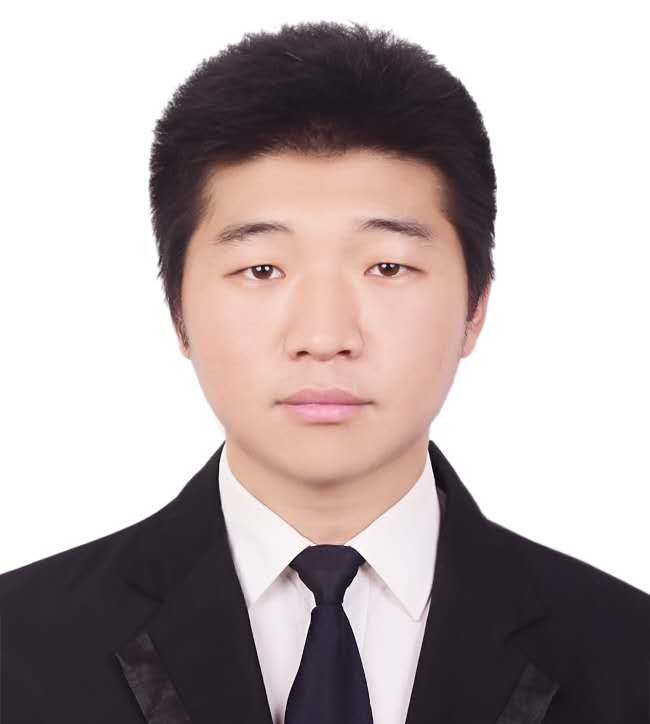
\includegraphics[width=1in]{profile}} & \scshape{高亚虎} & {Linux~}\progressbar{0.55} \\
    & \email{gao\_yahu@163.com} & {C~}\progressbar{0.45} \\
    & \phone{(+86) 131-2029-0626\ \ \ \ \ \ } & {Python~}\progressbar{0.45} \\
    & \github[github.com/yahugao]{https://github.com/yahugao} & {Java~}\progressbar{0.2}
  \end{tabu}
}

\section{\faCogs\ 项目经验}\normalsize
\datedsubsection{\textbf{微博立场检测}, FlyAI竞赛平台}{2020年07月15日 -- 2020年09月08日}
\datedsubsection{\textbf{智能问答系统}, FlyAI竞赛平台}{2020年07月15日 -- 2020年09月08日}
检索式问答系统,基于tf-idf对句子进行相似度计算,
\datedsubsection{\textbf{知识图谱}, 阿里云天池竞赛平台}{2020年07月15日 -- 2020年09月08日}
\datedsubsection{\textbf{新闻文本分类}, 阿里云天池竞赛平台}{2020年07月15日 -- 2020年09月08日}
\begin{itemize}
\item{训练集为对按照字符级别进行匿名处理的新闻数据,共有14个类别,20W样本,测试集为2W条样本。分别使用SVM、Naive Bayes、FastText、CNN、RNN、RCNN和HAN对训练集进行了拟合。以F1-score为衡量标准,SVM的效果最好达到了0.924, 其次为HAN得分为0.896. 对HAN模型进行了添加卷积层、使用动态学习率、早停、改变词嵌入维度、向其中的LSTM添加dropout并改变输出维度的调整,以缓解模型过拟合。}
\end{itemize}

\section{\faCogs\ 知识与技能}\normalsize
\begin{itemize}
  \item {熟悉文本表征BOW和TF-IDF, 词表征one-hot和word2vec, 了解ELMo和Bert}
  \item {熟悉LSTM, 了解传统的机器学习算法LR、SVM、DT和神经网络模型CNN、RNN、RCNN、FastText、HAN}
  \item {了解并具有keras和Pytorch的使用经验; 能熟练使用Emacs、Vim和Git; 熟悉Linux系统, 了解Linux系统的基本结构和文件系统。}
  \end{itemize}

\section{\faUsers\ 个人经历}\normalsize
\datedsubsection{\textbf{瞬联软件科技有限公司}\ 系统工程师}{2017年09月 -- 2019年11月}
\begin{itemize}
\item {参与WindRiver Linux系统的研发与测试,主要负责涉及文件系统相关的问题。在bug无法复现时结合堆栈信息和内核源码定位并修复问题; 对系统中涉及的CVE漏洞进行监控和修复。曾根据堆栈信息, 修复了三周复现一次的文件系统bug。}
 \item {因妻子需要出国访学一年,不放心,故辞职陪读。}
\end{itemize}
% \section{\faUsers\ 实习经历}
\datedsubsection{\textbf{英特尔(中国)有限公司}\ 实习软件工程师}{2016年8月 -- 2017年2月}
\begin{itemize}
\item {完成了LTP(Linux test project)由PC端向移动端的移植与验证,解决了LTP在平台迁移过程中的不兼容问题, 向LTP开源社区成功提交了修复数据类型的patch。}
\end{itemize}
% \section{\faGraduationCap\  教育背景}
\datedsubsection{\textbf{中国人民解放军信息工程大学}\ 硕士研究生:\ 计算机科学与技术}{2014年9月 -- 2017年7月}
\begin{itemize}
\item {研究方向为软件分析与逆向工程,期间发表学术论文两篇(知网检索一篇), 学位论文一篇。}
\end{itemize}

\datedsubsection{\textbf{河北理工大学(现华北理工大学)}\ 本科:\ 计算机科学与技术}{2010年9月 -- 2014年7月}
\vspace{1ex}
\section{\faInfo\ 其他}
% increase linespacing [parsep=0.5ex]
\begin{itemize}\normalsize
  \item {两年的bug修复经验,养成了工作认真,思维严谨的好习惯。自学机器学习和自然语言处理,具有良好的自我驱动学习能力。平时喜欢健身和跑步,身体健康。}
  \end{itemize}
  
\end{document}

%%% Local Variables:
%%% mode: latex
%%% TeX-master: t
%%% End:
